\documentclass[../ai_in_finance]{subfiles}
\usepackage[margin=1in]{geometry}
\usepackage{tikz}
\usetikzlibrary{positioning}
\usepackage{amsmath}
\usepackage{amssymb}
\usepackage{booktabs}
\usepackage{eurosym}
\usepackage{floatrow}
\usepackage{draftwatermark}

\SetWatermarkText{WSuo@Queensu.ca}
\SetWatermarkScale{1.4}
\SetWatermarkColor{gray!35}
\SetWatermarkAngle{45}

\usepackage{makeidx}
\makeindex

\begin{document}

\chapter{Financial Markets, Institutions, and Instruments}

\section{Introduction}

Financial markets are the institutions through which capital is allocated, risk is transferred, and prices are discovered. They allow households to save, firms to finance investment, governments to fund spending, and investors to diversify exposure. A solid understanding of these markets is essential for anyone who wants to use data science or artificial intelligence in finance, because the objects of analysis are not abstract numbers but real contracts, incentives, and trading mechanisms.

In a broad sense, modern finance is built on a simple but powerful idea: people do not all have the same preferences, opportunities, or time horizons. Some agents want to consume today, others want to save for the future, and still others are willing to accept risk in exchange for compensation. Financial markets provide the mechanisms that connect these different needs. Without such markets, savings would be less productive, firms would find it harder to grow, and risk would be harder to manage.

This chapter introduces the basic structure of financial markets and the major classes of financial instruments. The discussion begins with the roles of institutions and participants, then moves to the major types of securities traded in modern markets, and finally explains how prices are formed in real trading systems. The goal is to provide a conceptual foundation that will be useful when later chapters examine pricing, portfolio management, risk, and trading strategies.

Three worked examples anchor the more mechanical sections of the chapter: a bid-ask spread decomposed into its adverse-selection and inventory-cost components, a hand-computed walk through a small limit order book showing exactly how an incoming order gets filled at one price or several, and a no-arbitrage bond-pricing example that shows what happens, concretely, when two ways of pricing the same cash flow disagree. A case study of the 2010 Flash Crash closes the chapter, tying the abstract mechanics of order flow and liquidity to a single, well-documented afternoon when they broke down in public.

The chapter's institutional material, who trades, what they trade, and where, builds the vocabulary that every later chapter assumes: Chapters 5 and 10 price and hold the debt, equity, and derivative instruments this chapter's ``Financial Instruments'' section catalogues, Chapters 11 and 12 return to the limit order book and price discovery mechanics worked through in Section~\ref{sec:order-book-example} at execution and then microsecond speed, and Section~\ref{sec:no-arbitrage}'s no-arbitrage logic recurs, in progressively more quantitative form, in every valuation and pricing chapter that follows.

Readers already comfortable with market structure may skim the descriptive sections, but the worked examples are used again later in the book and are worth working through by hand at least once.

\section{Why Financial Markets Exist}\index{Why Financial Markets Exist}

A financial market exists because economic agents have different needs and different time horizons. A household may wish to save for retirement, a firm may need funding for expansion, and a government may require resources to finance public projects. These parties do not all have the same opportunities or preferences. Markets create a mechanism for matching supply and demand for capital.

The role of a financial market is therefore not limited to moving money from one person to another. Markets also allow people to shift risk across time and across states of the world. For example, a farmer who fears a decline in crop prices can use a futures contract to lock in a sale price. A pension fund that wants stable long-term income can purchase government bonds. A young entrepreneur who needs capital to build a company can issue equity to investors who are willing to share the upside and downside of the venture.

Financial markets also provide information. Prices do not only reflect current supply and demand; they also encode expectations about future cash flows, interest rates, inflation, and corporate performance. As a result, financial markets are not merely venues for exchange. They are systems for aggregating dispersed information and converting it into prices that guide decisions.

For this reason, a market becomes more useful when participants can trade quickly and with confidence. Liquidity, transparency, and regulation matter. If a market is illiquid, prices may be unstable and trading costs may be high. If it lacks transparency, participants may face information asymmetry and make poor decisions. If it lacks rules, trust can erode and market participants may withdraw from the system.

\section{Who Participates in Financial Markets}\index{Who Participates in Financial Markets}

Financial markets are populated by a diverse set of participants, each with different objectives and constraints. Households and retail investors often save for retirement, education, or other future needs. Firms issue securities to raise funding for investment. Governments borrow to finance public spending or manage budget imbalances. Financial institutions such as banks, mutual funds, pension funds, and insurers intermediate between those who provide capital and those who need it. Chapter 1's Table 1.5 previewed these participant roles at a glance; this section develops each one in more depth.

Market makers play a particularly important role. A market maker provides liquidity by standing ready to buy and sell securities, usually quoting both a bid price and an ask price. In return for taking on inventory risk and exposure to adverse price movements, market makers earn the spread between the two prices. This spread is a measure of trading cost, but it is also a compensation for providing immediacy and continuity to the market.

Arbitrageurs and hedge funds also influence market behavior. Arbitrageurs seek to exploit pricing discrepancies across related assets or markets. Hedge funds often pursue more complex strategies that may involve leverage, short selling, or macroeconomic views. Their activity can improve pricing efficiency, but it also can increase volatility when markets are under stress.

Finally, regulators and central banks shape the environment in which markets operate. Regulators enforce rules on disclosure, conduct, and market integrity. Central banks influence short-term interest rates and can intervene in crises to support liquidity or stabilize the financial system. For this reason, market outcomes are not determined only by private incentives; they also depend on public policy.

\section{Major Financial Institutions}\index{Major Financial Institutions}

Financial markets are organized around institutions that perform specialized functions. Banks provide lending services, facilitate payments, and transform maturity and liquidity profiles. Asset managers collect capital from investors and allocate it across portfolios of securities. Insurance companies pool risk by charging premiums in exchange for compensation when specified losses occur. Exchanges provide venues where orders can be matched, and central clearinghouses reduce counterparty risk by interposing themselves between buyers and sellers. Chapter 1's Table 1.3 summarized these institutions' roles at a glance; this section develops each one further.

These institutions have different business models and incentives. A commercial bank, for example, earns money by borrowing at one rate and lending at another. An asset manager earns fees by managing assets on behalf of clients. An insurance company earns premiums and invests the proceeds while managing claims. Each institution therefore faces unique risks, including credit risk, market risk, liquidity risk, and operational risk.

The financial system is fragile when institutions become highly interconnected. A bank may lend to a hedge fund, which may trade derivatives with a broker, which may depend on short-term funding from another bank. Interconnections can make the system more efficient under normal conditions, but they can also transmit shocks quickly during periods of stress. This is one reason why understanding institutions is essential for understanding financial crises.

The interaction between these institutions and the broader economy is profound. When banks tighten credit, firms may reduce investment. When insurers become more cautious, certain risks may become harder to insure. When exchanges improve market structure, trading costs may fall and liquidity may improve. These changes are not merely technical. They affect real economic activity, corporate decisions, and household welfare.

\section{Financial Instruments: The Core Contracts}\index{Financial Instruments: The Core Contracts}

Financial instruments are the contracts that are traded in markets. They can be classified in several broad categories, including debt securities, equity securities, derivatives, and alternative instruments. Each category serves a different economic purpose, and each has its own pricing logic. Chapter 1's Table 1.4 previewed the markets these instruments trade in; the rest of this section develops each instrument type in depth.

\subsection{Debt Securities}\index{Debt Securities}

Suppose a government wants to build a highway that will benefit taxpayers for decades but costs more than this year's tax revenue can cover, or a corporation wants to build a factory that will not turn a profit until it is finished. Both need a way to raise a large sum of money now against a promise to repay it, with something extra, over time, and both need that promise to be tradable, so that whoever lends the money today is not stuck holding an illiquid IOU for thirty years if their own circumstances change.

Debt securities are the financial technology that solves this problem: a bond is a standardized, tradable loan, where the investor buying it lends money to the issuer in exchange for a stream of future payments and the eventual repayment of principal at maturity. Bonds can be issued by governments, corporations, or other entities, and each issuer carries a different level of credit quality.

Government bonds are often viewed as relatively safe, though they still carry interest-rate risk and inflation risk. Corporate bonds generally offer higher yields because they are exposed to default risk. The pricing of bonds is closely related to the time value of money and discounting. A bond with a fixed coupon becomes more valuable when market interest rates fall and less valuable when rates rise. This is why bond prices and yields move inversely.

The bond market is also important because it provides a benchmark for the broader economy. Long-term government bond yields are often interpreted as signals of expected future growth and inflation. In this sense, bond markets are not only mechanisms for financing; they are also tools for interpreting macroeconomic conditions.

\subsection{Equity Securities}\index{Equity Securities}

A bond is a poor fit for a very different kind of firm: one whose value lies almost entirely in an uncertain future, a startup that might be worth nothing or might be worth billions, with no stable stream of cash flow today from which to make fixed interest payments at all. Locking such a firm into a bond's rigid repayment schedule could bankrupt it during a lean year even if its long-run prospects remain excellent.

Equity securities solve this by letting investors share directly in the firm's fortunes rather than lending against a fixed promise: they represent ownership claims in firms, and a common stock share gives the holder a claim on future profits and, in many cases, a vote in certain corporate matters. Equity investors are residual claimants, meaning they are paid only after other obligations, such as debt payments, have been satisfied. As a result, equities are generally riskier than bonds but offer the possibility of greater upside.

The valuation of stocks is more complicated than that of bonds because future dividends and firm value are uncertain. Investors often use dividend discount model\index{dividend discount model (DDM)}s, earnings-based valuation, or relative valuation approaches. In all cases, the underlying logic is that the value of an equity claim depends on expectations about future cash flows and the discount rate. A stock that promises strong future growth may command a high price even if current profits are modest.

Equity markets are also important because they provide a way for firms to raise permanent capital. Unlike debt, which requires contracts and scheduled payments, equity does not have a contractual maturity. This flexibility makes equity attractive for firms that expect growth, but it also means that shareholders bear more uncertainty than lenders.

\subsection{Derivatives}\index{Derivatives}

Neither a bond nor a stock, on its own, lets a wheat farmer lock in today what price they will receive for a harvest still six months from being planted, or lets an airline protect itself against a jet-fuel price spike without actually buying and storing barrels of oil it has nowhere to put. What both need is a contract whose payoff is tied to something else's future price, without requiring either party to own that underlying asset outright in the meantime.

Derivatives are exactly this: contracts whose value depends on the performance of another asset or variable. Common examples include forwards, futures, options, and swaps. A forward contract obligates the buyer and seller to exchange an asset at a future date for a predetermined price. A futures contract performs a similar role but is standardized and traded on an exchange. An option gives the holder the right, but not the obligation, to buy or sell an asset at a specified price before or at a certain date.

Derivatives are used for hedging, speculation, and arbitrage. A producer may use futures to lock in a selling price. A portfolio manager may use options to protect against downside risk. A trader may use derivatives to express a view on volatility or market direction. Because derivatives often embed leverage, they can magnify gains and losses, which makes them important tools for both risk management and risk creation.

The economic importance of derivatives is difficult to overstate. By allowing parties to transfer risk more precisely, they expand the range of risk management strategies available to firms and investors. However, they can also create hidden exposures if participants misunderstand their payoff structure. This is one reason why derivatives are closely monitored by regulators and risk managers.

\subsection{Swaps}\index{Swaps}

Suppose a company has already issued floating-rate debt, so its interest payments rise and fall with market rates, but its own revenue is stable and predictable, and it would much rather know exactly what it owes each quarter than gamble on where rates go next. Reissuing the debt itself, paying off the old loan and negotiating a brand-new fixed-rate one, would be slow, expensive, and might not even be possible if the lender is unwilling to renegotiate.

A swap solves this without touching the underlying loan at all: it is an agreement between two parties to exchange cash flows according to a pre-specified formula, and the most common type by far is the interest rate swap.

In a plain-vanilla interest rate swap, one party pays a fixed rate on a notional principal amount while the other pays a floating rate, historically tied to LIBOR\index{LIBOR}, a benchmark discontinued after regulators found panel banks had manipulated it and replaced by transaction-based Alternative Reference Rates\index{Alternative Reference Rates (ARRs)} such as the Secured Overnight Financing Rate (SOFR)\index{Secured Overnight Financing Rate (SOFR)} in the U.S., with only the net difference actually changing hands. Critically, the notional principal itself is never exchanged; it exists only to determine the size of the interest payments.

Swaps are used primarily to change the interest rate exposure of an existing position without altering the underlying asset or liability. A company that has issued floating-rate debt but prefers the predictability of fixed payments can enter a swap to pay fixed and receive floating, effectively converting its floating-rate liability into a fixed-rate one from a cash-flow perspective. A pension fund seeking to match long-dated fixed liabilities might do the reverse. Currency swaps, credit default swaps (which transfer credit risk rather than interest-rate risk, the same credit risk measured directly with the default-probability and loss models of Chapter 9), and total return swaps extend this same basic idea, exchanging one set of cash flows for another, to other kinds of risk.

Swaps trade almost entirely over-the-counter rather than on exchanges, which historically made the market for them opaque; post-2008 reforms, discussed later in this chapter, pushed much of the standardized swap market toward centralized clearing specifically to reduce the kind of counterparty risk concentration that swaps had exposed during the financial crisis.

\subsubsection*{A Worked Example: Valuing an Existing Interest Rate Swap}

A plain-vanilla interest rate swap can be valued as the difference between two bonds: the fixed leg is valued exactly like a coupon bond, discounting each fixed payment plus a final notional repayment, while the floating leg, because its coupon resets to the prevailing market rate at each reset date, is worth par (its notional value) at any reset date, regardless of what has happened to interest rates since the swap began. Consider a two-year swap with a \$10 million notional and a fixed rate of $5\%$, agreed some time ago, being valued today, immediately after a reset, when the current one-year and two-year discount rates are $4\%$ and $4.5\%$ respectively, lower than the $5\%$ fixed rate locked in at initiation. The fixed leg's annual coupon is $0.05 \times 10{,}000{,}000 = \$500{,}000$, so its present value is
\begin{equation*}
PV_{\text{fixed}} = \frac{500{,}000}{1.04} + \frac{500{,}000 + 10{,}000{,}000}{1.045^2} \approx \$10{,}095{,}933.72,
\end{equation*}
while the floating leg, valued at par immediately after its reset, is worth exactly $PV_{\text{floating}} = \$10{,}000{,}000$. The swap's value to the party paying fixed and receiving floating is
\begin{equation*}
V_{\text{fixed payer}} = PV_{\text{floating}} - PV_{\text{fixed}} = 10{,}000{,}000 - 10{,}095{,}933.72 \approx -\$95{,}933.72,
\end{equation*}
a loss to the fixed-rate payer, and an equal and opposite gain to the floating-rate payer, since market rates have fallen since the swap was struck, leaving the fixed-rate payer locked into paying $5\%$ when the market now says $4$--$4.5\%$ is fair. This is precisely the mechanism by which an existing swap's mark-to-market value changes over its life without either counterparty doing anything at all: pure movement in market interest rates redistributes value between the two legs, exactly the same discounting logic Chapter 5 applies to bond pricing, applied here to the difference of two cash flow streams rather than a single one.

\subsection{Other Instruments}\index{Other Instruments}

Other instruments include money market securities, preferred shares, mortgage-backed securities, and exchange-traded funds. These products illustrate the breadth of modern finance. Some are designed for short-term liquidity management, while others combine exposure to many assets in a single tradable instrument. Exchange-traded funds, in particular, have become widely used because they offer diversification and low-cost access to broad market exposure.

The growth of index funds and exchange-traded funds has changed the structure of investing. Instead of selecting individual securities, many investors now buy broad baskets of assets that track an index. This shift has lowered costs, increased market participation, and changed the nature of price formation in some markets. It also shows that modern finance is not only about individual securities; it is also about packaging and distributing risk efficiently.

An exchange-traded fund's price is kept close to the value of its underlying holdings through a creation-and-redemption mechanism: authorized institutional participants can exchange a basket of the underlying securities for new ETF shares, or vice versa, whenever the ETF's market price drifts far enough from its net asset value to make doing so profitable. This arbitrage-like mechanism, similar in spirit to the no-arbitrage logic in Section~\ref{sec:no-arbitrage}, is what keeps an ETF tracking its underlying index closely under normal conditions, though it can break down during periods of severe stress if the underlying securities themselves become difficult to trade.

\section{How Markets Are Organized}\index{How Markets Are Organized}

Markets are not all structured in the same way. Some are organized as exchanges with centralized order books, while others are over-the-counter markets where participants trade directly with one another. In exchange-traded markets, buyers and sellers submit orders that are matched according to price and time priority. In over-the-counter markets, contracts are negotiated bilaterally and may be tailored to specific needs.

The distinction matters because it affects liquidity, transparency, counterparty risk, and transaction costs. Exchange-traded products are often easier to price and monitor, while over-the-counter trades may offer flexibility but require more careful risk management. For example, an exchange-listed stock can usually be traded quickly at a visible price, whereas a bespoke derivative contract may require negotiation, credit assessment, and collateral arrangements.

The study of these rules is called market microstructure. Even small changes in execution rules, fees, or order types can have meaningful effects on the quality of price discovery. A limit order, for example, may provide price improvement but may also fail to execute. A market order may execute immediately but at the cost of adverse price impact. These tradeoffs are central to both trading and research in finance.

A useful simple measure of trading cost is the bid-ask spread\index{bid-ask spread}:

\begin{equation*}
\text{Spread} = P_{\text{ask}} - P_{\text{bid}}.
\end{equation*}

This spread captures the cost of immediacy. When the spread is narrow, trading is cheaper and liquidity is stronger. When the spread is wide, the market is less liquid and the cost of trading is higher. For quantitative researchers, such quantities are often as important as the asset's return itself because they determine the practical profitability of a strategy.

\section{A Worked Example: Walking the Limit Order Book}\index{Walking the Limit Order Book}
\label{sec:order-book-example}

The bid-ask spread only describes the price of trading a single share. In practice, a limit order book\index{limit order book} lists multiple price levels on both sides, and a large order can ``walk'' through several levels, receiving a progressively worse average price. Table~\ref{tab:order_book} shows a simplified order book for a stock.

\begin{table}[htbp]
\centering
\caption{A simplified limit order book}
\label{tab:order_book}
\begin{tabular}{lrr@{\hspace{1.2cm}}lrr}
\toprule
\multicolumn{3}{c}{Asks (sell orders)} & \multicolumn{3}{c}{Bids (buy orders)} \\
\cmidrule(r){1-3} \cmidrule(l){4-6}
Level & Price & Size (shares) & Level & Price & Size (shares) \\
\midrule
1 & \$50.10 & 100 & 1 & \$50.05 & 150 \\
2 & \$50.15 & 200 & 2 & \$50.00 & 250 \\
3 & \$50.20 & 300 & 3 & \$49.95 & 200 \\
\bottomrule
\end{tabular}
\end{table}

The best bid is \$50.05 and the best ask is \$50.10, so the quoted bid-ask spread is \$0.05, consistent with the formula above. Figure~\ref{fig:order_book_depth} draws the same book as a depth chart, the standard way a trading desk actually visualizes it. Now suppose a trader submits a market buy order for 250 shares, more than the 100 shares available at the best ask. The order first consumes all 100 shares at \$50.10, then the remaining 150 shares at the next level, \$50.15:
\begin{equation*}
\text{Average execution price} = \frac{100(50.10) + 150(50.15)}{250} = \frac{5{,}010 + 7{,}522.50}{250} = \$50.13.
\end{equation*}
This average price is \$0.03 above the best ask of \$50.10, roughly 6 basis points of price impact, purely a consequence of order size relative to the liquidity available at each price level, with no new information entering the market at all. A trader who needs to buy or sell a large position faces exactly this tradeoff: submitting the entire order at once guarantees immediate execution but at a worse average price, while breaking the order into smaller pieces over time (the subject of the execution algorithms in Chapter 11) can reduce price impact at the cost of exposing the trader to price movements while the order is worked.

\begin{figure}[htbp]
\centering
\begin{lrbox}{\bookmeasuredbox}
    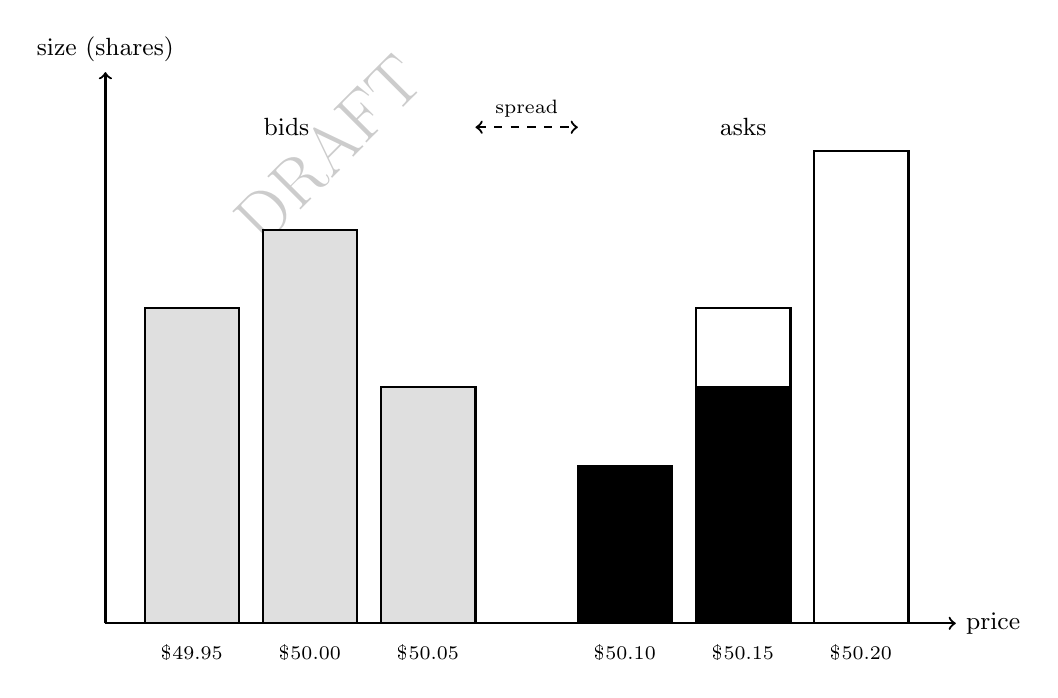
\begin{tikzpicture}[thick]
        \draw[->] (-0.5,0) -- (10.3,0) node[right,font=\small] {price};
        \draw[->] (-0.5,0) -- (-0.5,7.0) node[above,font=\small] {size (shares)};
        \draw[fill=gray!25] (0,0) rectangle (1.2,4.0);
        \draw[fill=gray!25] (1.5,0) rectangle (2.7,5.0);
        \draw[fill=gray!25] (3.0,0) rectangle (4.2,3.0);
        \node[below,font=\scriptsize] at (0.6,-0.15) {\$49.95};
        \node[below,font=\scriptsize] at (2.1,-0.15) {\$50.00};
        \node[below,font=\scriptsize] at (3.6,-0.15) {\$50.05};
        \draw[fill=black] (5.5,0) rectangle (6.7,2.0);
        \draw[fill=black] (7.0,0) rectangle (8.2,3.0);
        \draw[fill=white] (7.0,3.0) rectangle (8.2,4.0);
        \draw[fill=white] (8.5,0) rectangle (9.7,6.0);
        \node[below,font=\scriptsize] at (6.1,-0.15) {\$50.10};
        \node[below,font=\scriptsize] at (7.6,-0.15) {\$50.15};
        \node[below,font=\scriptsize] at (9.1,-0.15) {\$50.20};
        \node[font=\small] at (1.8,6.3) {bids};
        \node[font=\small] at (7.6,6.3) {asks};
        \draw[<->,dashed] (4.2,6.3) -- (5.5,6.3);
        \node[above,font=\scriptsize] at (4.85,6.3) {spread};
    \end{tikzpicture}
\end{lrbox}
\ifdim\wd\bookmeasuredbox<0.65\linewidth
\setlength{\bookcapwidth}{0.65\linewidth}
\else
\setlength{\bookcapwidth}{\wd\bookmeasuredbox}
\fi
\ffigbox[\bookcapwidth]{
\usebox{\bookmeasuredbox}
}{
    \caption{The limit order book of Table~\ref{tab:order_book} as a depth chart. Bid sizes (light gray) sit left of the spread, ask sizes (white outline) right; the solid black portion of the two lowest ask levels marks what the 250-share market order consumes.}
    \label{fig:order_book_depth}
}
\end{figure}

\section{Decomposing the Bid-Ask Spread}\index{Decomposing the Bid-Ask Spread}

The bid-ask spread is not pure profit for a market maker; it compensates for at least three distinct costs, and understanding the decomposition helps explain why spreads widen in some conditions and narrow in others.
\begin{itemize}
    \item \textbf{Order-processing cost}: the operational cost of handling a trade, which is largely fixed regardless of market conditions.
    \item \textbf{Inventory-holding cost}: compensation for the risk a market maker bears by holding a non-zero position while waiting for an offsetting order to arrive, discussed further in Section~\ref{sec:market-making}.
    \item \textbf{Adverse-selection cost}: compensation for the risk of trading with a counterparty who has better information, since an informed trader will systematically pick off stale quotes.
\end{itemize}
A trade price bounces back and forth between the bid and the ask as buy and sell orders arrive, even when nothing about the asset's underlying value has changed at all: a trade at the ask followed by a trade at the bid looks, in the raw price series, exactly like the price falling and then recovering, so a wider spread mechanically produces larger, more frequent back-and-forth price changes. Roll's (1984) implied spread estimator\index{Roll's implied spread model} turns this bounce into a measurement tool, recovering the effective spread purely from observed price changes, without ever seeing the order book itself,
\begin{equation*}
\text{Spread} \approx 2\sqrt{-\text{Cov}(\Delta P_t, \Delta P_{t-1})},
\end{equation*}
using the fact that this bid-ask bounce induces exactly the kind of negative autocorrelation in consecutive price changes that the covariance term inside the square root captures. This is a useful reminder for the time series methods of Chapter 7: not every statistical pattern in price data reflects economically meaningful predictability, some of it is a direct, mechanical consequence of market microstructure.

\section{The Economics of Price Discovery}\index{Economics of Price Discovery}

Financial prices are the output of a complex process in which participants with different information and objectives update their beliefs. A stock price may rise because investors revise their expectations of future cash flows, because risk premiums change, or because a large buyer enters the market. The same price change can have multiple interpretations, which is why finance is both quantitative and interpretive.

Because prices are affected by information, incentives, and trading frictions, they do not always move smoothly. Sudden price movements can reflect news, uncertainty, algorithmic trading, or liquidity shocks. In the short run, prices may deviate from fundamental values because of temporary imbalance or limited liquidity. In the long run, however, competition and arbitrage tend to push prices toward values consistent with available information and economic fundamentals.

This is why economists and practitioners distinguish between fundamentals and short-run market dynamics. A fundamental analyst asks what an asset ought to be worth given expected cash flows and risk. A market microstructure analyst asks how trading rules and order flow shape the observed price path. Both perspectives are necessary for a complete understanding of finance.

Understanding price discovery is also important for AI applications in finance. A predictive model may identify patterns in observed prices, but without an understanding of the market mechanism behind those prices, the model may misinterpret noise as signal. The best applications of machine learning in finance combine statistical learning with economic and institutional insight. A model that predicts price movements may still fail if it ignores transaction costs, market impact\index{market impact}, and changing liquidity conditions.

\section{Why Market Structure Matters for Quantitative Finance}\index{Why Market Structure Matters for Quantitative Finance}

The practical relevance of this chapter becomes clear when one considers how financial models are used in the real world. A portfolio manager does not merely choose assets based on expected return and risk. The manager must also consider how easily those assets can be bought or sold, how much price impact trading will create, and whether the strategy can survive transaction costs.

The same logic applies to credit risk models, fraud detection systems, and forecasting algorithms. A model that performs well on historical data may still fail in real trading if it ignores the institutional setting in which decisions are implemented. This is why finance is not simply a data problem. It is a problem of data, incentives, constraints, and execution.

For quantitative readers, this point is especially important. Statistical methods can be powerful, but they are most useful when paired with an understanding of the underlying market mechanism. The most successful applications of AI in finance are not those that treat markets as a black box. They are those that combine rigorous modeling with financial intuition.

A concrete illustration makes this abstract point specific. Suppose a machine learning model identifies a statistical pattern predicting that a small-cap stock will outperform over the next week, based purely on historical price and volume data.

Before acting on this signal, a quantitatively sophisticated practitioner asks several institutional questions that the model itself cannot answer: How wide is the bid-ask spread for this stock, and does the expected outperformance exceed the round-trip cost of trading it, using the spread decomposition introduced later in this chapter? How much of the stock's average daily volume would the intended position represent, and would establishing that position via the order-book mechanics described in Section~\ref{sec:order-book-example} move the price enough to erode the expected gain? Is the stock easy to borrow if the strategy requires shorting, and are there restrictions on short selling of small-cap names during periods of stress?

None of these questions are visible in the historical price data the model was trained on, yet each one can determine whether a statistically significant signal is also an economically exploitable one. This is the precise sense in which market structure, not just statistical significance, determines whether a trading idea survives contact with a real market.

\section{Money Markets, Capital Markets, and the Lifecycle of a Trade}\index{Money Markets, Capital Markets, and the Lifecycle of a Trade}

Financial markets are often divided into money markets and capital markets. Money markets are used for short-term borrowing and lending, typically for maturities of less than one year. They include instruments such as Treasury bills, commercial paper, certificates of deposit, and repurchase agreements. These markets are crucial for liquidity management because banks, corporations, and governments frequently need to finance short-term obligations or invest excess cash for a brief period. Chapter 1's Table 1.4 previewed money markets alongside equity, bond, derivatives, and foreign exchange markets; this section and Chapter 5 develop each of these further.

Capital markets, by contrast, are used for long-term financing. They include equity and long-term debt markets, and they are central to funding business investment and public infrastructure. A firm that wishes to expand production may issue long-term bonds or equity. A government may issue sovereign debt to finance roads, schools, or defense spending. In both cases, the capital market allows the financing decision to be separated from the immediate cash position of the issuer.

Another useful distinction is between primary and secondary markets. In a primary market, new securities are issued for the first time. In a secondary market, existing securities are traded among investors. The primary market raises funds for the issuer, while the secondary market determines the price at which securities are traded after issuance. The existence of a liquid secondary market is important because it reduces uncertainty for investors and makes it easier for firms to issue securities in the first place.

The lifecycle of a trade illustrates the practical importance of market structure. A trader or investor first decides to buy or sell an asset. The order is routed through a broker to an exchange or an over-the-counter dealer. If the market is electronic and highly liquid, the order may be executed almost immediately. If the market is more fragmented or less liquid, the order may be partially filled or may require price concessions. Once the trade is complete, settlement occurs, which means that ownership is transferred and cash is exchanged. In many markets, settlement is not instantaneous; it may take a few days. During this period, counterparty and operational risk remain relevant.

This process is not purely mechanical. It reflects the interaction of incentives, technology, and regulation. For instance, high-frequency trading firms may compete to offer the best execution speed, while institutional investors may prioritize minimizing market impact. A retail investor may value simplicity and lower cost, whereas a hedge fund may be willing to bear more risk for a chance at a strategic advantage. All of these objectives interact within the same marketplace.

The repurchase agreement\index{Repurchase Agreement (Repo)}, or repo, deserves particular attention among money market instruments because of the central role it plays in the plumbing of the financial system. In a repo, one party sells a security, typically a government bond, to another party while simultaneously agreeing to repurchase it at a slightly higher price on a specified future date, often the very next day. Economically, this is a collateralized short-term loan: the cash borrower posts the security as collateral, and the difference between the sale and repurchase price is the effective interest rate, known as the repo rate.

Banks, hedge funds, and other institutions rely on the repo market to fund large securities positions on a daily basis, which means that a disruption in repo markets, as occurred at several points during the 2008 crisis, can rapidly force institutions to sell assets they would otherwise have held, transmitting stress across the financial system in exactly the way described in the systemic risk discussion below.

Concretely, suppose a dealer needs to borrow $\$10{,}000{,}000$ overnight and posts Treasury securities as collateral in exchange for cash at an annualized overnight repo rate of $5\%$. Using the money market convention of a 360-day year, the interest owed for one day is
\begin{equation*}
\$10{,}000{,}000 \times 0.05 \times \frac{1}{360} = \$1{,}388.89,
\end{equation*}
so the dealer repurchases the collateral the next day for $\$10{,}001{,}388.89$. This tiny per-day interest amount, applied to an enormous notional and rolled over every business day, is exactly why even a small rise in overnight repo rates, of the kind observed in September 2019 when repo rates briefly spiked well above the Federal Reserve's target range, can signal a meaningful shortage of cash available for this kind of short-term collateralized lending.

Settlement conventions are a second detail with outsized practical importance. Most equity markets settle trades on a T+1 or T+2 basis (one or two business days after the trade date), meaning that ownership and cash do not actually change hands at the moment a trade is agreed. This gap creates counterparty risk, the possibility that the other side of the trade fails to deliver cash or securities as promised, which is precisely the risk that the clearinghouses discussed in the next section exist to mitigate.

\section{The Business of Exchanges and Market Data}\index{Business of Exchanges and Market Data}

It is easy to think of an exchange purely as neutral infrastructure, a venue where buyers and sellers meet, without asking how the exchange itself makes money. In practice, modern exchanges are for-profit businesses with several distinct revenue streams, and understanding them explains a number of features of market structure that would otherwise seem arbitrary.

Listing fees are charged to companies for the right to have their shares traded on a given exchange, and they give exchanges an incentive to attract high-quality, high-volume issuers. Transaction fees are charged per trade, often under a ``maker-taker'' model in which an exchange pays a small rebate to participants who post resting limit orders (adding, or ``making,'' liquidity) and charges a slightly larger fee to participants whose orders execute immediately against those resting orders (removing, or ``taking,'' liquidity). This fee structure is a direct, deliberate subsidy for market-making activity, and it materially affects the profitability calculations of the market makers discussed in Section~\ref{sec:market-making}.

Market data fees are a third, increasingly significant revenue source: exchanges sell real-time price and order-book data to trading firms, and the most detailed, lowest-latency feeds command substantial premiums over the free or delayed data available to retail investors. Finally, co-location fees, charging trading firms for the right to place their own servers physically inside or adjacent to the exchange's data center, directly monetize the speed advantage discussed in the technology and market design material later in this chapter; a firm that pays for co-location receives information about order flow and executes its own orders with lower latency than a firm trading from a remote location, purely as a function of the physical distance data must travel.

These revenue streams matter for a quantitative reader for two reasons. First, they explain why exchanges have strong commercial incentives to attract high-frequency trading activity specifically, since such activity generates outsized transaction and data-fee revenue relative to its economic footprint, which is part of the broader political and regulatory debate about whether current market structure appropriately balances the interests of high-frequency participants against those of long-term investors. Second, they are a reminder that the market data used throughout this book, and assumed to arrive at negligible cost in every worked example so far, is itself a commercial product whose cost, coverage, and latency vary enormously depending on how much a firm is willing to pay, a practical constraint that shapes what kind of strategy is even feasible for a given research budget.

\section{Clearing, Settlement, and Systemic Risk}\index{Clearing, Settlement, and Systemic Risk}

Once a trade is executed, the market must ensure that the agreement is honored. Clearing refers to the process of determining obligations between counterparties, while settlement refers to the final exchange of cash and securities. In exchange-traded markets, a clearinghouse often acts as the central counterparty, guaranteeing the trade if one side defaults. This reduces bilateral credit risk, but it also creates a new concentration of risk in the clearinghouse itself.

The importance of clearing and settlement becomes most obvious during periods of stress. If many participants are forced to liquidate positions at once, the system may face liquidity shortages and margin calls. A small shock can therefore propagate through the network of institutions that depend on one another for financing and collateral. This is the core idea behind systemic risk: the failure of one institution or market segment can quickly undermine the stability of the broader financial system.

The 2008 global financial crisis showed how quickly seemingly isolated problems could become systemic. Mortgage defaults in the United States spread through securitization structures, derivatives markets, and funding markets, eventually affecting banks, insurers, and governments around the world. The lesson was not simply that risk had been mispriced, but that the financial system had become highly interconnected and insufficiently transparent. The crisis also highlighted the importance of regulations on leverage, capital, and liquidity.

A central clearinghouse manages its own concentrated risk primarily through margin requirements: each clearing member must post collateral, called initial margin, sized to cover the clearinghouse's potential loss if that member defaults under plausible adverse price moves, and must post additional variation margin daily (or, during volatile periods, intraday) to cover losses on open positions as prices move. This mechanism protects the clearinghouse, but it also means that a sharp, sudden price move can trigger simultaneous margin calls across many participants at once, forcing coordinated selling precisely when the market is least able to absorb it, a dynamic that played a visible role in the Flash Crash\index{Flash Crash of 2010} case study later in this chapter and in various episodes of the 2008 crisis.

Clearinghouses have themselves become large enough, and interconnected enough with their member banks, that regulators now treat major clearinghouses as systemically important institutions in their own right, subject to their own capital and risk-management standards.

Variation margin differs from the initial-margin mechanics of Section~\ref{sec:short-selling-margin} in one important respect: rather than being called only once a position breaches a maintenance threshold, it is settled to zero at the end of every trading day, marking every open position to its current market price.

Suppose a trader buys one stock-index futures contract with a notional value of $\$50{,}000$ and posts an initial margin of $\$5{,}000$ ($10\%$ of notional). If the index falls $2\%$ that day, the trader's mark-to-market loss is $0.02 \times \$50{,}000 = \$1{,}000$, reducing the margin balance to $\$5{,}000 - \$1{,}000 = \$4{,}000$; the clearinghouse issues a variation margin call for exactly $\$1{,}000$ to restore the balance to $\$5{,}000$ before trading resumes the next day. Because this settlement happens daily rather than only at a maintenance-breach threshold, losses on a futures position never accumulate silently the way they can in the stock-margin example above, but it also means that a clearing member with many leveraged futures positions faces a new, and potentially large, daily cash obligation every time the market moves sharply against it, which is precisely the liquidity-drain mechanism this section's systemic-risk discussion refers to.

Table~\ref{tab:margin_comparison} summarizes the two margin mechanics side by side, since it is easy to conflate them despite their different timing and trigger conditions.

\begin{table}[htbp]
\centering
\begin{lrbox}{\bookmeasuredbox}
\begin{tabular}{lll}
\toprule
& Short-sale margin (Section~\ref{sec:short-selling-margin}) & Futures variation margin \\
\midrule
Counterparty & Broker & Central clearinghouse \\
Settlement frequency & Only when a threshold is breached & Every trading day \\
Trigger & Equity falls below maintenance \% & Any price move, however small \\
Typical use case & Individual equity short position & Standardized futures and swaps \\
\bottomrule
\end{tabular}
\end{lrbox}
\ifdim\wd\bookmeasuredbox<0.65\linewidth
\setlength{\bookcapwidth}{0.65\linewidth}
\else
\setlength{\bookcapwidth}{\wd\bookmeasuredbox}
\fi
\ttabbox[\bookcapwidth]{
\usebox{\bookmeasuredbox}
}{
\caption{Two margin mechanisms compared: bilateral broker margin on a short sale versus centrally cleared futures margin.}
\label{tab:margin_comparison}
}
\end{table}

\section{Regulation, Disclosure, and Market Integrity}\index{Regulation, Disclosure, and Market Integrity}

Markets require rules because they involve trust, information, and incentives. Without regulation, participants may exploit others through fraud, insider trading, or manipulation. Disclosure requirements help investors evaluate firms and make informed decisions. Capital and liquidity rules reduce the chance that institutions will become insolvent or unable to meet obligations during stress. Market surveillance systems detect suspicious behavior and support confidence in the fairness of the trading process.

The balance between free markets and regulation is a persistent theme in finance. Too little regulation may encourage excessive risk-taking and misconduct. Too much regulation may reduce innovation and impose unnecessary compliance costs. The most effective regulatory frameworks are therefore designed to protect integrity and stability while preserving the ability of markets to allocate capital efficiently.

From the perspective of AI and data science, regulation also matters because it shapes the data environment. Financial institutions must report certain information, comply with auditing standards, and provide transparent records. These requirements create rich datasets that can be used for forecasting, fraud detection, and risk analysis. At the same time, regulatory constraints limit what can be done with the data, especially when privacy, fairness, or market abuse concerns are involved.

A few specific regulatory frameworks are worth knowing by name because they recur throughout the rest of this book.

\begin{itemize}
    \item \textbf{The Securities and Exchange Commission (SEC)} oversees U.S. securities markets and disclosure.
    \item \textbf{Regulation NMS}\index{Regulation NMS (Reg NMS)} (National Market System) governs how orders are routed and executed across competing U.S. exchanges, directly shaping the market microstructure discussed throughout this chapter.
    \item \textbf{The Dodd-Frank Act}\index{Dodd-Frank Act}, passed in 2010 in response to the 2008 financial crisis, introduced the central clearing requirements for standardized swaps mentioned above, along with the Volcker Rule\index{Volcker Rule} restricting proprietary trading by banks, and stress-testing requirements for large financial institutions that are directly relevant to the risk models in Chapters 8 and 9.
    \item \textbf{MiFID II}\index{MiFID II} (the Markets in Financial Instruments Directive), in Europe, imposes extensive transparency and best-execution requirements on trading venues and investment firms.
    \item \textbf{Basel III}\index{Basel Accords}\index{Basel III} is an international framework setting minimum capital and liquidity requirements for banks, intended to make the banking system more resilient to exactly the kind of interconnected shocks described in the systemic risk discussion above.
\end{itemize}

None of these frameworks is a topic this book covers in depth, but recognizing their names and general purpose is useful context for the compliance-related material in Chapter 13.

\section{The Link Between Market Structure and AI}\index{Link Between Market Structure and AI}

A modern AI system in finance cannot be designed as if markets were simple, frictionless, and fully observable. Real markets have heterogeneous participants, delayed information, hidden inventory, and strategic behavior. For example, an algorithm that trades based on price patterns may perform well in a calm market but fail in a stressed market where liquidity evaporates and spreads widen. A credit model that uses historical repayment data may become less reliable if underwriting standards change or if the economy enters a new regime.

This is why financial machine learning should be interpreted as an engineering problem embedded in an economic environment. The model is one component of a broader system that includes data pipelines, risk controls, execution logic, and compliance procedures. The same prediction can have very different consequences depending on how it is used. A recommendation that is harmless in a research setting may be dangerous in a live trading environment if it creates concentration risk or triggers herding behavior.

The chapter therefore closes with a practical lesson: the most valuable AI applications in finance are those that respect the structure of the market. They use data carefully, incorporate financial theory, and are evaluated not only by predictive accuracy but by their economic and operational consequences.

This connection between market structure and AI runs in both directions, and it is worth being explicit about the second direction as well. So far this section has emphasized how market structure constrains and shapes AI systems; AI systems, in turn, have themselves become part of the market structure they operate within.

The high-frequency market-making firms discussed later in this chapter increasingly rely on machine learning to set quotes and manage inventory risk in real time. Large asset managers use natural language processing, the subject of Chapter 14, to parse earnings calls and regulatory filings faster than human analysts could. Exchanges themselves use anomaly-detection systems, related to the fraud-detection methods of Chapter 13, to flag potentially manipulative trading patterns for regulatory review. This means that the ``other participants'' referred to throughout this chapter, whose behavior shapes liquidity, spreads, and price discovery, are themselves increasingly AI systems, and their collective behavior is part of what any new AI system entering the market must anticipate and adapt to.

This observation has a subtle but important consequence for model validation. A backtest evaluates a strategy against historical data generated by the market as it existed in the past, including the mix of human and automated participants active at that time. If a meaningful share of that historical liquidity and price-setting behavior came from other algorithms that have since been retired, upgraded, or replaced, then the market a new strategy will actually face going forward may behave differently from the market reflected in its backtest, not because of any change in economic fundamentals, but because the population of participants generating prices has itself changed. This is a more subtle version of the non-stationarity concern raised in Chapter 1 and developed further in Chapter 6, and it is specific to markets with a high degree of algorithmic participation.

\section{Liquidity, Leverage, and the Economics of Market Making}\index{Liquidity, Leverage, and the Economics of Market Making}
\label{sec:market-making}

Liquidity is one of the most important but least visible features of financial markets. A liquid market allows participants to trade quickly without moving the price too much. In practice, liquidity is a multidimensional concept:

\begin{itemize}
    \item \textbf{Depth} is the volume that can be traded at a given price.
    \item \textbf{Immediacy} is the speed with which an order can be executed.
    \item \textbf{Resiliency} is the speed with which the market returns to a stable state after a shock.
    \item \textbf{Tightness} is the narrowness of the bid-ask spread.
\end{itemize}

A market with high liquidity is often easier to use for hedging, investment, and risk management, because traders can enter and exit positions more cheaply.

Market makers, introduced earlier in this chapter as participants who quote both a bid and an ask and earn the spread between them, do more than passively post two prices: they actively absorb temporary imbalances between buy and sell orders, buying when others want to sell and selling when others want to buy. This is where the inventory risk mentioned earlier actually bites. If the market maker purchases an asset and its price falls, the position loses value. If the market maker sells short and the price rises, losses can also accumulate quickly. The willingness of market makers to bear this risk is therefore central to market functioning.

Market-making decisions are shaped by information asymmetry. When informed traders possess better information than others, market makers face adverse selection. An informed trader who knows that an asset is likely to rise may be more likely to buy, while an informed trader who knows that an asset is likely to fall may be more likely to sell. The market maker, who does not know whether a trade conveys good or bad information, may respond by widening spreads and reducing participation. This mechanism is one reason why trading costs often rise in periods of uncertainty.

Leverage is another essential concept in this setting. A trader who borrows funds to increase position size can magnify gains, but can also magnify losses. Margin requirements are designed to reduce the chance that a leveraged position becomes too large relative to the trader's equity. When prices move against the position, a margin call may force liquidation. That forced selling can amplify price movements and create additional stress in the market. This is why leverage, while useful for efficient investment and speculation, is also a source of instability when risk management is weak.

\section{A Worked Example: Short Selling and Margin Calls}\index{Short Selling and Margin Calls}
\label{sec:short-selling-margin}

Leverage and margin are easiest to understand through a concrete short sale. Suppose a trader believes a stock currently priced at $\$50$ is overvalued and borrows $100$ shares to sell short, receiving proceeds of $100 \times \$50 = \$5{,}000$. Under a typical initial margin requirement of $150\%$ of the value of the position (the U.S. Regulation T standard), the trader must maintain total account equity of at least $1.5 \times \$5{,}000 = \$7{,}500$: the $\$5{,}000$ in short-sale proceeds plus an additional $\$2{,}500$ of the trader's own cash deposited as margin.

As the stock price $P$ moves, the trader's liability, the cost of buying back the $100$ borrowed shares, is $100P$, while total account equity remains the fixed $\$7{,}500$ credit balance minus that liability:
\begin{equation*}
\text{Equity}(P) = 7{,}500 - 100P.
\end{equation*}
A broker typically requires a maintenance margin of at least $25\%$ of the current value of the short position, meaning $\text{Equity}(P)/100P \geq 0.25$. Setting this ratio equal to exactly $0.25$ and solving for $P$ gives the price at which a margin call is triggered:
\begin{equation*}
7{,}500 - 100P = 0.25(100P) \quad\Longrightarrow\quad 7{,}500 = 125P \quad\Longrightarrow\quad P = \$60.
\end{equation*}
At $P=\$60$, the trader's liability has grown to $100 \times \$60 = \$6{,}000$ while equity has fallen to $\$7{,}500 - \$6{,}000 = \$1{,}500$, exactly $25\%$ of the $\$6{,}000$ liability, confirming the calculation. A price increase of only $20\%$, from $\$50$ to $\$60$, is enough to trigger a margin call on a position that started with $150\%$ initial margin, illustrating precisely how leverage compounds a short seller's losses: the loss on the position itself is $\$1{,}000$, but it consumes $\$1{,}000$ out of only $\$2{,}500$ of the trader's own capital, a $40\%$ loss on equity from a $20\%$ adverse price move. If the trader cannot deposit additional funds once the call is issued, the broker will buy back some or all of the borrowed shares on the trader's behalf, often at whatever price is available, which is exactly the kind of forced selling into a moving market described in this chapter's Flash Crash case study and, at the scale of an entire highly leveraged fund rather than a single position, in the LTCM episode discussed later in this chapter.

\section{A Simple No-Arbitrage Example}\index{Simple No-Arbitrage Example}
\label{sec:no-arbitrage}

A useful way to understand why prices in finance are constrained by structure is to consider a very simple arbitrage argument. Suppose an investor can buy a one-period risk-free bond that costs $100$ and pays $105$ one year later. The risk-free interest rate implied by this bond is

\begin{equation*}
r = \frac{105 - 100}{100} = 0.05.
\end{equation*}

Now suppose there is also a claim that pays one unit of money with certainty in one year. If the claim were priced at $0.95$ today, then an investor could buy the claim for $0.95$ and receive $1$ next year. This is equivalent to earning a return of about $5.26\%$, which is higher than the risk-free rate available from the bond. In that case, rational investors would buy the claim and sell the bond, pushing prices back into line. The no-arbitrage principle says that two assets with the same payoff must have the same price, otherwise investors can create a riskless profit. This is a foundational idea behind pricing in derivatives, fixed income, and many broader valuation applications.

This example may appear simple, but it illustrates a powerful principle. Financial prices are not arbitrary; they are linked by the logic of replication and absence of arbitrage. A quantitative analyst should therefore be careful not to interpret a model output in isolation. If a model predicts a price that violates basic consistency conditions, it may be signaling an error in the model, a missing constraint, or an overlooked transaction cost. This is one reason why financial modeling is both statistical and economic.

The same logic extends to more complex instruments such as options, swaps, and structured products. In these cases, the challenge is often to identify the relevant replicating portfolio and the correct discounting process. The existence of such relationships is what makes finance a systematic discipline rather than a purely descriptive one. Even when markets appear noisy, there are still strong forces that keep valuations tied to economic logic.

A second example, this time for a forward contract, makes the same point using a replicating portfolio rather than a single comparison bond. Suppose a stock trades today at $S_0 = \$100$, pays no dividends over the next year, and the risk-free rate is $r = 5\%$. A one-year forward contract obligates its holder to buy the stock in one year at a price fixed today; the no-arbitrage forward price is
\begin{equation*}
F_0 = S_0(1+r) = 100(1.05) = \$105,
\end{equation*}
the cost of replicating the forward's payoff by borrowing $\$100$ today at the risk-free rate, buying the stock now, and holding it for one year (a strategy known as cash-and-carry).

If the forward instead traded in the market at $F_{\text{mkt}} = \$110$, an arbitrageur could borrow $\$100$, buy the stock, and simultaneously sell (go short) the forward at $\$110$; in one year, the arbitrageur delivers the stock against the forward for $\$110$, repays the loan plus interest of $100(1.05) = \$105$, and keeps a riskless profit of $\$110 - \$105 = \$5$ regardless of where the stock price actually ends up, since the forward sale fixes the delivery price in advance. This is precisely the type of relationship Chapter 5's option and derivative pricing methods generalize: an option's value, unlike a forward's, depends on the underlying's volatility because the option's payoff is not a fixed, symmetric obligation, but the same replication logic, construct a portfolio of tradable assets with an identical payoff, and price the derivative to match, underlies both.

\subsection*{A Third Example: Triangular Arbitrage in Currency Markets}\index{Triangular Arbitrage}

No-arbitrage pricing applies just as directly when three related prices, rather than two, must be mutually consistent, and foreign exchange markets provide the cleanest illustration. Three exchange rates, EUR/USD, GBP/USD, and EUR/GBP, are not independent: knowing any two implies the no-arbitrage value of the third, since converting EUR to USD and then USD to GBP must produce the same result as converting EUR to GBP directly. Suppose the market quotes $\text{EUR/USD} = 1.10$ (one euro buys \$1.10) and $\text{GBP/USD} = 1.25$ (one pound buys \$1.25), implying a no-arbitrage $\text{EUR/GBP}$ rate of
\begin{equation*}
\frac{\text{EUR/USD}}{\text{GBP/USD}} = \frac{1.10}{1.25} = 0.88,
\end{equation*}
one euro should be worth $\pounds0.88$. If the EUR/GBP market instead directly quotes $0.87$, euros are priced slightly cheaper against pounds directly than the USD route implies, and a triangular arbitrage exists: starting with $\pounds1{,}000{,}000$,
\begin{align*}
\text{Step 1 (GBP} \to \text{EUR at } 0.87\text{):} &\quad 1{,}000{,}000 / 0.87 \approx \text{\euro}1{,}149{,}425.29, \\
\text{Step 2 (EUR} \to \text{USD at } 1.10\text{):} &\quad 1{,}149{,}425.29 \times 1.10 \approx \$1{,}264{,}367.82, \\
\text{Step 3 (USD} \to \text{GBP at } 1/1.25\text{):} &\quad 1{,}264{,}367.82 \times 0.80 \approx \pounds1{,}011{,}494.25,
\end{align*}
a riskless profit of about $\pounds11{,}494$, or roughly $1.15\%$, on the round trip, realized in seconds and requiring no view whatsoever on whether any of the three currencies will rise or fall. Exactly as in the bond and forward examples above, this mispricing cannot persist: high-frequency and algorithmic traders (the subject of Chapters 11 and 12) monitor exactly this kind of three-way consistency continuously, and the resulting arbitrage trading pushes the three rates back into alignment within moments of any deviation appearing, which is precisely why triangular arbitrage opportunities in liquid, major-currency pairs are typically too small and short-lived to exploit manually, existing today mainly as a textbook illustration of a real economic force rather than a realistically accessible trading strategy for anyone without a fully automated, low-latency system.

Although financial theory often uses idealized assumptions, real markets are full of frictions. These frictions include transaction costs, taxes, delays, information asymmetry, margin requirements, and limits on borrowing. A frictionless market would make it easy to buy and sell any asset at a known price, but real markets are not like that. The presence of frictions changes the economics of investment and the behavior of prices.

For example, if trading a security is expensive, an investor may need a larger expected return to justify holding it. If borrowing is restricted, a trader cannot always implement a strategy that would otherwise be profitable. If information is not shared equally, some participants may act faster or more intelligently than others. These realities matter because even small frictions can have large effects in the aggregate, particularly when many participants are trading at the same time.

This is why practitioners often distinguish between theoretical prices and realized prices. Theoretical models may suggest that two assets with identical cash flows should trade at the same value. In practice, they may not if short-selling is difficult, if settlement is delayed, or if the market is temporarily illiquid. Such deviations create opportunities for some participants, but they also create risk for others. This tension between theory and practice is one of the defining features of finance.

\section{Financial Crises, Contagion, and Resilience}\index{Financial Crises, Contagion, and Resilience}

A complete understanding of financial markets also requires an understanding of crises. Crises are not random accidents. They often emerge when leverage is high, liquidity is fragile, and institutions are highly interconnected. In such conditions, a seemingly small shock can trigger forced selling, margin calls, and sudden changes in funding conditions. The result can be a cascade of losses that spreads across firms, asset classes, and countries.

This general pattern, high leverage, fragile liquidity, and deep interconnection combining to turn a seemingly small shock into a cascade, is exactly what played out in the 2008 financial crisis, already discussed earlier in this chapter's treatment of clearing and systemic risk: mortgage defaults, amplified through securitization, derivatives, and short-term funding markets, became a systemic event precisely because institutions that seemed healthy on the surface turned out not to be resilient once funding dried up.

For AI and quantitative finance, this lesson is important. A model can be accurate under normal conditions and still fail in crisis periods if the underlying regime changes. The data may be nonstationary, the relationship between variables may weaken, and trading strategies may become far more costly to execute. This is why model stress testing\index{stress testing} and scenario analysis are essential in practice.

An earlier episode, the near-collapse of the hedge fund Long-Term Capital Management (LTCM)\index{Long-Term Capital Management (LTCM)} in 1998, illustrates a related but distinct lesson: sophisticated quantitative models can fail specifically because of leverage and crowding, not because the underlying statistical reasoning was wrong. LTCM's strategies relied on historical relationships between related securities converging back to normal levels, a reasonable premise most of the time, applied with very high leverage to turn small, reliable-looking spreads into large returns.

When the 1997 Asian financial crisis and 1998 Russian debt default triggered a broad flight to safety, the specific historical relationships LTCM depended on moved sharply against it, and because many other market participants held similar positions, there was no way to exit without pushing prices even further in the wrong direction. The fund's near-failure was severe enough that the Federal Reserve organized a private-sector bailout to prevent broader market disruption. The lesson for quantitative finance is not that statistical models are unreliable, but that a model's estimated relationships can break down precisely when many market participants are relying on the same relationship and using leverage to size their bets on it, a crowding risk that a model built purely from historical price data will rarely reveal on its own.

\section{Technology, Speed, and Market Design}\index{Technology, Speed, and Market Design}

The design of financial markets has changed dramatically with technology. Electronic trading, co-location, and automation have reduced costs and increased the speed at which orders can be processed. This has improved access for many participants, but it has also increased complexity. The market now resembles a digital system in which algorithms interact with each other at high speed and where small delays can be extremely valuable.

Technology therefore changes not only the efficiency of trading but also the structure of competition. A participant with faster infrastructure may gain an edge even if its economic view is not superior. This explains why market microstructure has become a central topic in modern finance. Price formation is no longer shaped only by fundamentals; it is also shaped by trading rules, network effects, and technological capabilities.

\section{Case Study: The 2010 Flash Crash}\index{2010 Flash Crash}

On May 6, 2010, U.S. equity markets experienced one of the most dramatic intraday moves in modern history: major indices fell sharply within minutes, with some individual stocks and exchange-traded funds briefly trading at absurd prices, pennies in some cases, before the market recovered most of its losses within the same session. The episode, subsequently known as the Flash Crash, is a useful case study precisely because the subsequent joint SEC-CFTC investigation identified a chain of mechanical, structural causes rather than any single piece of adverse economic news.

The investigation traced the initial trigger to a large sell order in E-mini S\&P 500 futures, executed by an automated algorithm designed to sell a fixed percentage of trading volume without regard to price or time. As this selling pressure pushed prices down, high-frequency trading firms, which had been providing a substantial share of market liquidity, began rapidly buying and reselling the same contracts to each other rather than absorbing the imbalance, a pattern sometimes described as ``hot potato'' trading.

Within minutes, many of these same high-frequency firms and other liquidity providers withdrew from the market entirely as their own risk controls triggered, causing depth (recall the liquidity dimensions introduced in Section~\ref{sec:market-making}) to evaporate almost completely on both the futures and underlying equity markets at once. With so little resting liquidity left in the order book, the arrival of ordinary sell orders was enough to walk prices down dramatically, exactly the mechanical price-impact effect illustrated numerically in Section~\ref{sec:order-book-example}, just at a much larger and faster scale.

The Flash Crash illustrates several themes from this chapter operating simultaneously. It shows that liquidity is not a fixed, guaranteed feature of a market but a behavior that participants can withdraw suddenly and simultaneously, especially under stress, exactly the regime-dependence of liquidity discussed in this chapter's challenges section below. It shows that automated systems interacting with other automated systems can produce dynamics, like the hot-potato pattern, that were not intended or anticipated by the designers of any individual system.

And it shows the practical consequence of market fragmentation across many linked trading venues and instruments: the crash originated in a futures contract but transmitted almost instantly to the equity market, since prices in closely related instruments are tied together by the same no-arbitrage forces introduced in Section~\ref{sec:no-arbitrage}. In direct response, regulators introduced market-wide circuit breakers and individual stock ``limit up-limit down'' rules designed to pause trading automatically during extreme price moves, a structural safeguard that did not exist in May 2010.

\section{Challenges in Modeling Market Structure}

The institutional detail covered in this chapter is not merely background; it creates specific, recurring challenges for anyone trying to build data-driven or AI-based systems on top of financial markets.

\textbf{Fragmented and opaque data.} A meaningful share of trading, especially in bonds, derivatives, and large institutional equity orders, occurs over-the-counter or through dark pools rather than on a single transparent exchange. Any dataset built from public exchange feeds alone is therefore an incomplete picture of the market, and models trained on it can miss where and how large trades actually occur.

\textbf{Microstructure noise.} At very short time horizons, prices are affected by the mechanics of trading itself, bid-ask bounce, order-book dynamics, and the strategic behavior of market makers, not just by fundamental information. A high-frequency model that treats every price tick as a fundamental signal risks fitting this microstructure noise rather than anything economically meaningful, a problem revisited in the chapters on high-frequency trading.

\textbf{Regime dependence of liquidity.} Liquidity, spreads, and market depth are not fixed properties of a security; they change with volatility, macroeconomic conditions, and market stress, often at exactly the moments when a trading or risk model most needs to work reliably. A backtest run only over calm periods can therefore substantially overstate a strategy's real-world performance.

\textbf{Reflexivity and adversarial dynamics.} Unlike a physical system, a market contains other participants who adapt their behavior in response to observed patterns, including patterns generated by other algorithms. A signal or arbitrage relationship, once discovered and traded upon at scale, can weaken or disappear, which means static, one-time model validation is not sufficient.

\textbf{Modeling systemic effects.} Individual asset-level or firm-level models rarely capture the network effects, interconnections between institutions, correlated leverage, shared counterparties, that drive systemic events such as the 2008 crisis. Building models that account for these system-wide dynamics remains a much harder and less mature area than single-asset prediction.

\textbf{Realistic transaction cost estimation.} As emphasized throughout this chapter, the profitability of a strategy depends heavily on execution costs, market impact, and available liquidity, none of which are fully known in advance and all of which are easy to underestimate in a backtest that assumes trades execute at the observed price with no impact.

Taken together, these challenges mean that a purely statistical view of market data, one that ignores the institutional structure described in this chapter, is unlikely to produce robust financial models. This is the central justification for treating market structure as foundational material before the book turns to prediction and optimization methods in later chapters.

\section{Key Takeaways}

Financial markets exist to allocate capital, transfer risk, and reveal information. Their institutions and instruments shape the opportunities and constraints faced by investors and firms. Debt, equity, and derivatives are the main building blocks of modern finance, and the way these instruments are traded has direct consequences for liquidity, pricing, and risk management. A careful understanding of market structure is therefore necessary before one can evaluate more advanced models or trading strategies.

The order-book example in Section~\ref{sec:order-book-example} made this concrete: even with no news and no change in fundamental value, a large order can move the average execution price simply because liquidity is finite at each price level, and the Flash Crash case study showed the same mechanism operating at a market-wide scale when liquidity providers withdrew simultaneously.

The swaps and regulatory material introduced in this chapter, interest rate swaps, Dodd-Frank, MiFID II, and Basel III, will resurface directly in the risk management chapter that follows, since modern risk management is defined as much by regulatory capital requirements as by statistical modeling choices.

The overall lesson to carry forward is that market structure is not a fixed backdrop against which trading happens; it actively shapes prices, costs, and the viability of any strategy built on top of it.

\section{Suggested Exercises}

\begin{enumerate}
    \item Explain the difference between a bond and a stock in terms of cash flow rights and risk.
    \item Describe the role of a market maker in a financial market.
    \item Give one example of how a derivative can be used for hedging.
    \item Explain why liquidity matters for asset prices.
    \item Compare exchange-traded and over-the-counter markets in terms of transparency and counterparty risk.
    \item Discuss one reason why a trading strategy might fail even if it has good historical predictive performance.
    \item Explain how a bid-ask spread reflects the cost of immediacy in a market.
    \item Choose one challenge from Section 3.22 (``Challenges in Modeling Market Structure'') and explain how it could cause a backtested trading strategy to look profitable historically but lose money in live trading.
    \item Using the order book in Table~\ref{tab:order_book}, compute the average execution price and price impact (in dollars and basis points) for a market sell order of 300 shares, which will walk through the bid side of the book.
    \item Explain, in your own words, the difference between the order-processing, inventory-holding, and adverse-selection components of the bid-ask spread, and give one market condition that would cause each component to widen.
    \item Explain why an interest rate swap does not require the exchange of the notional principal amount, and describe a situation in which a firm would want to swap from floating-rate to fixed-rate interest payments.
    \item Compare the 2008 financial crisis and the LTCM episode described in this chapter: what role did leverage play in each, and how did the two episodes differ in their trigger and their transmission mechanism?
    \item Using Section~\ref{sec:short-selling-margin}'s method, a trader shorts 200 shares at \$80 with a $150\%$ initial margin requirement and a $30\%$ maintenance margin. Compute the total initial account equity and the share price at which a margin call is triggered.
    \item Using Section~\ref{sec:no-arbitrage}'s cash-and-carry logic, a non-dividend-paying stock trades at \$40 and the risk-free rate is $4\%$. Compute the no-arbitrage one-year forward price, and describe the specific trades an arbitrageur would execute today and in one year if the forward instead traded at \$43.
    \item A dealer borrows \$25 million overnight in the repo market at an annualized rate of $4.5\%$, using the 360-day money-market convention from this chapter's repo example. Compute the dollar interest owed for one night and the total repurchase price.
    \item Explain how the Flash Crash illustrates the ``regime dependence of liquidity'' challenge from Section 3.22, using specific details from the case study.
    \item Using this chapter's interest rate swap example, recompute the swap's value to the fixed-rate payer if the one-year and two-year discount rates were instead $5.5\%$ and $6\%$ (rates have risen above the $5\%$ fixed rate rather than fallen below it), and explain in words why the sign of the swap's value to the fixed-rate payer flips relative to the original example.
    \item Using this chapter's triangular arbitrage example, suppose the EUR/GBP rate is instead quoted at $0.89$ rather than $0.87$ (EUR/USD and GBP/USD unchanged). Determine whether the arbitrage cycle described in the text ($\pounds \to \text{\euro} \to \$ \to \pounds$) is still profitable, and if not, describe which direction around the triangle would now be profitable instead.
\end{enumerate}

\section{Further Reading}

For readers who want to study these topics in more depth, the following books are especially useful:

\begin{itemize}
    \item Bodie, Kane, and Marcus, \emph{Investments}. A broad introduction to markets, instruments, and institutions that complements this chapter's overview with a fuller treatment of portfolio and asset-pricing theory.
    \item Hull, \emph{Options, Futures, and Other Derivatives}. The standard reference for the derivatives instruments introduced briefly in this chapter, developing their pricing and hedging in full in Chapter 5.
    \item Fabozzi, \emph{Fixed Income Analysis}. Goes well beyond this chapter's brief bond-market coverage into the pricing, risk, and institutional detail of fixed-income securities.
    \item Shleifer, \emph{Inefficient Markets}. A behavioral-finance counterpoint to the efficient-market and price-discovery discussion in this chapter, examining the frictions and limits to arbitrage that keep prices from always reflecting fundamentals.
    \item O'Hara, \emph{Market Microstructure Theory}. The foundational academic treatment of the order-book mechanics, bid-ask spread decomposition, and market-making economics introduced in this chapter's worked examples.
\end{itemize}

\end{document}
